\documentclass[12pt]{paper}
\usepackage[margin=1in]{geometry}
\usepackage{float}
\usepackage{natbib}
\bibliographystyle{apsr}
\usepackage{graphicx}
\graphicspath{ {../fig/} }
\usepackage{setspace}
\usepackage[super]{nth}
\usepackage{booktabs}
\usepackage{makecell}
\usepackage{amsmath}
\usepackage{dcolumn}
%\usepackage{authblk}
\usepackage{hyperref}
\usepackage{wrapfig}
\usepackage{amsmath}
\usepackage{adjustbox}
\usepackage{hanging}
%\usepackage{etoolbox}
%\AtBeginEnvironment{quote}{\singlespacing\small}

\newlength{\cslhangindent}
\setlength{\cslhangindent}{1.5em}
\newenvironment{cslreferences}%
{\setlength{\parindent}{0pt}%
	\everypar{\setlength{\hangindent}{\cslhangindent}}\ignorespaces}%
{\par}

\title{Structural Topic Modeling for Studying White Nationalism Online}
\author{Sarah R. Warren}
\date{}

\begin{document}
\maketitle
%\thispagestyle{empty}
%\clearpage
%\setstretch{1}

\doublespacing
\section*{Introduction}
Over the past five years, mainstream American politics has seen a distinct rise in white-nationalist and neo-Nazi activity. From the Unite the Right rally in Charlottesville, Virginia in 2017 to the White Civil Rights Rally in Washington, D.C. in 2018, these events sparked renewed concern and interest in white nationalism, which is notable because many Americans believe the United States has virtually eradicated racism (Krysan and Moberg 2016). In a society that has operated under the illusion of postracialism for so long, these attacks and the seemingly-overnight popularity of white nationalism was particularly surprising. These events raise several important questions for scholars of political violence. In particular, who are the white nationalists of the 21st Century? How are they mobilizing and what set of ideas are they mobilizing around? In the digital age, how are they leveraging the Internet to their advantage? The answers to these questions not only inform us about white nationalists, but help us understand them in the context of the digital age.

To address these questions about white nationalists in the mass public, we need an environment in which scientists can observe their behavior, thoughts, and feelings, but where they do not know they are being directly observed. This is critical, because observation is likely to alter speech in the case of socially undesirable ideas (Nederhof 1985). The small body of work on white nationalists who are not public figures focuses on exclusively on their online communities or the spreading of “digital hate” on websites like Reddit and Twitter (Daniels 2018; Berlet and Mason 2019), but these platforms have strict content restrictions. Users expressing white supremacy are frequently banned and alt-right subreddits are frequently deleted. While this is normatively desirable insofar as it stifles hate-groups' ability to proselytize, it inhibits our understanding of \textit{what} these communities are saying and \textit{how} they are saying it.

To circumvent this kind of selection bias without violating these platforms’ Terms of Service by retaining deleted content, this paper presents a novel dataset of posts from StormFront.org, the largest white nationalist forum on the internet. This paper presents the dataset, which is publicly available for use and replication,  and endeavors to address the questions above by offering one of the first in-depth examinations of non-elite white nationalist ideology and rhetoric (for other examples, see: Thompson 2001; Wojcieszak 2010; and Hartzell 2020). 

To preview my results, I find that the majority of posts are under 1,000 words in length and forum activity spiked around the 2008 election of Barack Obama. Public activity on the forum has since declined, perhaps due to the creation of private groups for members only, which I discuss in Section III. I estimate a 60-topic Structural Topic Model (STM) from the full corpus of posts and find that the most prevalent topic is comprised of unigrams regarding nationalism, socialism, and ideology. Somewhat surprisingly, the next most-prevalent topic seems to focus on community; words like ``support" drive this topic. Language about race and white nationalism (often denoted ``wn" in forum shorthand) don't appear until the eighth-most prevalent topic. Further, sentiment analysis reveals forum language to be dominated by positive sentiment, followed by negativity, trust, and fear. These results appear to belie the ambivalence individual posters express about their ``white activism." On one hand, they express familial closeness and solidarity with their fellow whites; on the other, they express a great sense of racial anxiety and fear of ``white genocide" at the hands of other races. The forum functions both as a welcoming communal space where white nationalists can express their socially unaccepted views about whiteness and advance their goal of a white ethnostate, while also serving as a sort of anxiety-airing house of mourning over supposed white genocide at the hands of liberal ideology and other races.

The rest of this paper proceeds as follows. Section I introduces the data-generating process and data collection procedure. It introduces the context in which the forum posts were produces and what they do and do not contain, providing context for how we should interpret their content. Section II considers the contents of forum posts, using Structural Topic Modeling (STM) to describe the topics discussed within and across threads. It further considers the affect of forum posts, using sentiment analysis to describe the sentiments associated with topics within and across subforums. Section III places these data in the context of the structure of the forum. Section IV concludes with a discussion and thoughts for future work.

\section{StormFront.org}
StromFront.org, which boasts that ``Every month is white history month," is dedicated to fostering discussion and community among white nationalists around the world. It is a typical virtual community insofar as it is characterized by in-group norms, strong enforcement of these norms by moderators, and a specific set of shared interests and values (De Koster and Houtman 2008; Bowman-Grieve 2009). It was created in 1995 by former Ku Klux Klan (KKK) leader Don Black and has been called the “first major hate site on the Internet.” In 2001, StormFront transitioned from a simple webpage to an interactive message board. By 2005, that forum had grown to over 40,000 registered members and Stormfront was independently ranked within the top 1 percent of all websites in terms of activity (Kim 2005). StormFront has since grown to hundreds of thousands of members and is the largest white nationalist website on the internet, boasting over 60,000 unique viewers a day.

White nationalism is a derivative of white supremacy which advocates for separation of the races, the creation of a white ethnostate, and the preservation of white racial hegemony (Kim 2005). White nationalists attempt to distinguish themselves from white supremacists, arguing that they are not fueled by hatred or bigotry, but rather a desire to protect and preserve white identity in a culture of white erasure. Many others (Meddaugh and Kay 2009; Hartzell 2020) have noted that StormFront users employ the dispassionate, academic rhetoric of ``reasonable racism" in an attempt to legitimize their viewpoints and distance themselves from notions of emotion-driven racial hatred. Indeed, the posting guidelines on StormFront.org ban the use of racial epithets and profanity, warning, ``Before you post anything, remember that words have consequences, both for you and others. This is true even if they're posted pseudonymously on a discussion board," (\textit{Welcome: Guidelines for Posting}). Given this, there is a surprising lack of hate speech on StormFront.org (Gilbert et al. 2018).

There is a paucity of scholarly work concerning StormFront.org. Often, it makes use of a small sample of interviews (De Koster and Houtman 2008) or rhetorical analysis of a handful of posts (Bowman-Grieve 2009; Hartzell 2020). Scholarship which does make use of large corpi of texts from the forum often uses it to \textit{categorize} behavior - for example, exploring the prevalence of hate speech (Gibert et al. 2018) or posting patterns in the Opposing Views Forum (Bright et al. 2022), which is open to guests and even translated into Spanish, Portuguese, and French for international visitors. This article, by contrast, not only introduces a novel dataset of StromFront.org forum posts, but offers the first in-depth contextualization of StormFront.org as a virtual space.

The data I present here were scraped on September 7, 2021 and come from the three most popular public-facing threads (National Socialism, Positive White Nationalism, and Conservatism) on the Ideology and Philosophy subforum as of the day of scraping. There are a total of 5,423 unique posts, including the full text of the post, the username of the poster, the date and time it was posted, the forum to which it was posted, and the length of the post in characters. Figure 1 shows post frequency on the forums over time. The majority of posts are under 1,000 words in length and forum activity spiked around the 2008 election of Barack Obama. It appears to be around this time (2008-2009) that private groups were created within the forum, which perhaps has contributed to the significant decline in forum activity since 2012.

\begin{figure} \centering
	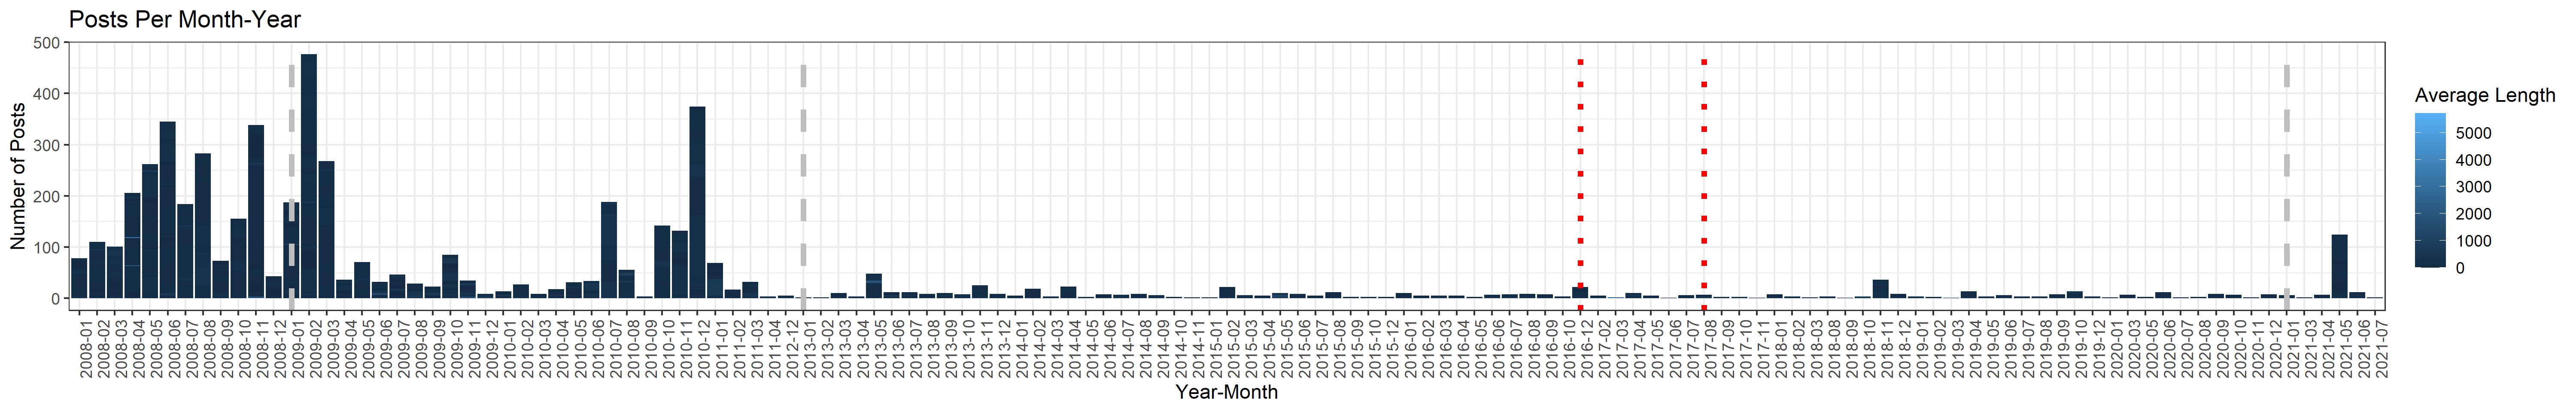
\includegraphics[width=.8\linewidth]{figs/ip_frequency_length.png}
	\caption{Post Prevalence and Length}
	\label{}
\end{figure}

Given the somewhat-public facing nature of the forum, I predict that the general content of the forum will be \textit{positive} and community focused. Topic modeling should reveal the underlying content of the corpus and sentiment analysis should reveal generally positive, communal sentiment.

\section{Empirical Analysis}
There is a paucity of academic work utilizing StormFront.org posts to study white nationalists. The small body of relevant academic research has largely focused on developing models and algorithms for \textit{categorizing} StormFront.org content (Gilbert et al. 2018). This article, in contrast, introduces a method to automatically identify topics (not categories) within forum posts based only on the specific reports being analyzed. Text classification is a form of supervised machine learning, in which a machine is fed a training set of labeled documents and is tasked with uncovering why each document is labeled as it is using document text. Topic modeling, by contrast, is a form of unsupervised learning, akin to clustering, where the set of topics are unknown \textit{a priori}.Topics represent latent structure in the corpus being analyzed. Categories represent a predetermined classification system which the machine learns and copies for new documents. Topics tell us what different pieces of texts are about; categories organize documents. Unlike categorization models, the topic-identification methodology used here does not rely on previously defined categories or training data and can be applied relatively rapidly by a single analyst.

I use structural topic modeling (STM) to uncover topics within the corpus of forum posts. STM is preferable in this context to Correlated Topic Models (CTM) and Latent Dirichlet Allocation (LDA) because STM allows topic prevalence and content to come from document metadata (Roberts et al. 2013). In substantive terms, this means that I can avoid LDA’s more restrictive assumptions - in particular, the assumption that all inference can be drawn from the document text alone. Because I know my data concern various topics under the umbrella of white nationalism, but know \textit{a priori} that different forums may use different language to express the same sentiment within the context of the forum, methods like CTM and LDA are suboptimal. Structural topic modeling allows me to draw inferences based on post metadata - such as the forum to which it was posted.

\begin{figure} \centering
	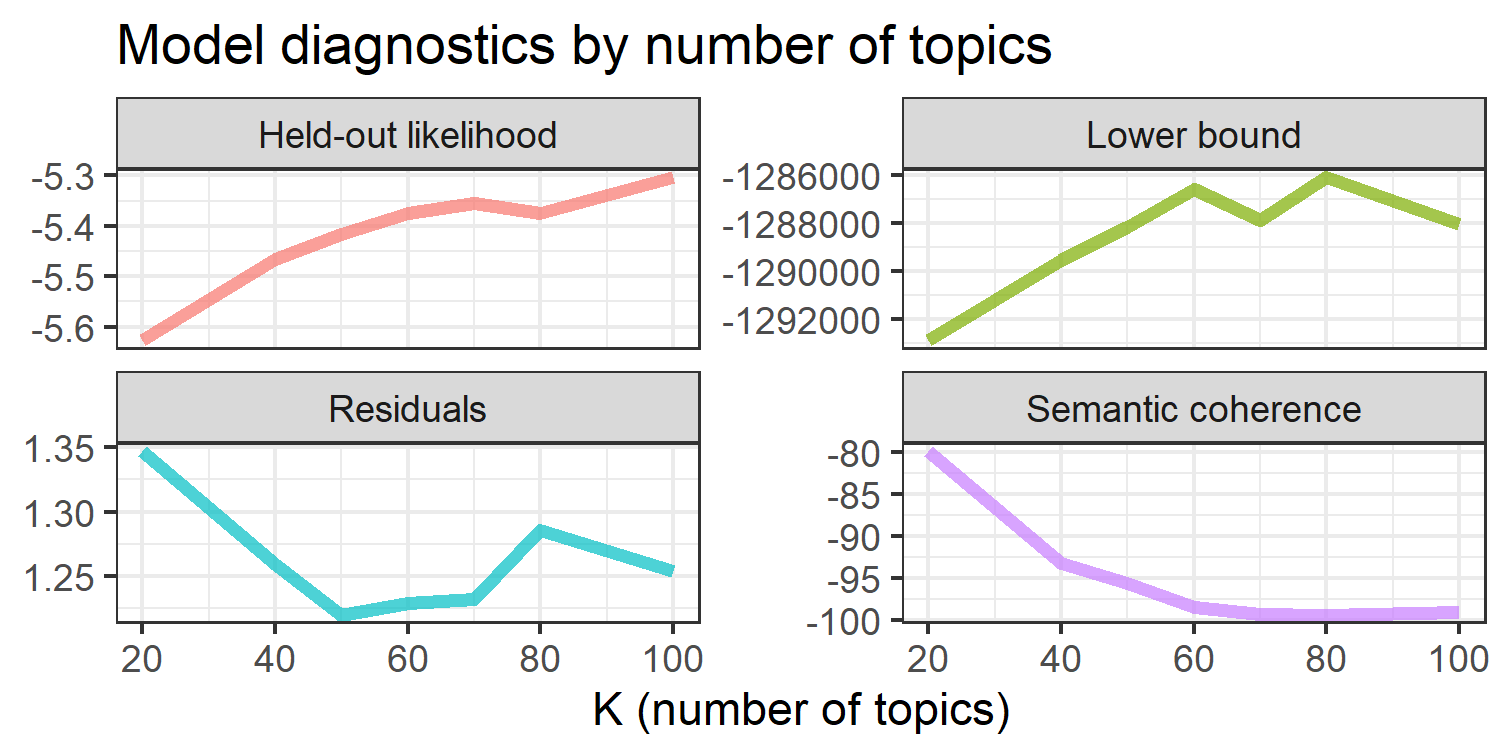
\includegraphics[width=.8\linewidth]{figs/diagnostics-by-topic.png}
	\caption{STM Results}
	\label{}
\end{figure}

I leverage the forum to which a text was posted to structure topic estimation. There is no way of knowing \textit{a priori} the appropriate number of topics to estimate, so I first estimated a series of 20, 50, 60, 80, and 100 topic models. The fit indices are shown in Figure 2. Ideally, the number of topics chosen will minimize the residuals and maximize the held-out likelihood. The basic idea of held-out likelihood is to hold out some fraction of the words in a set of documents, train the model and use the document-level latent variables to evaluate the probability of the held-out portion. By these metrics, a 60-70 topic model looks most appropriate. 

\begin{figure} \centering
	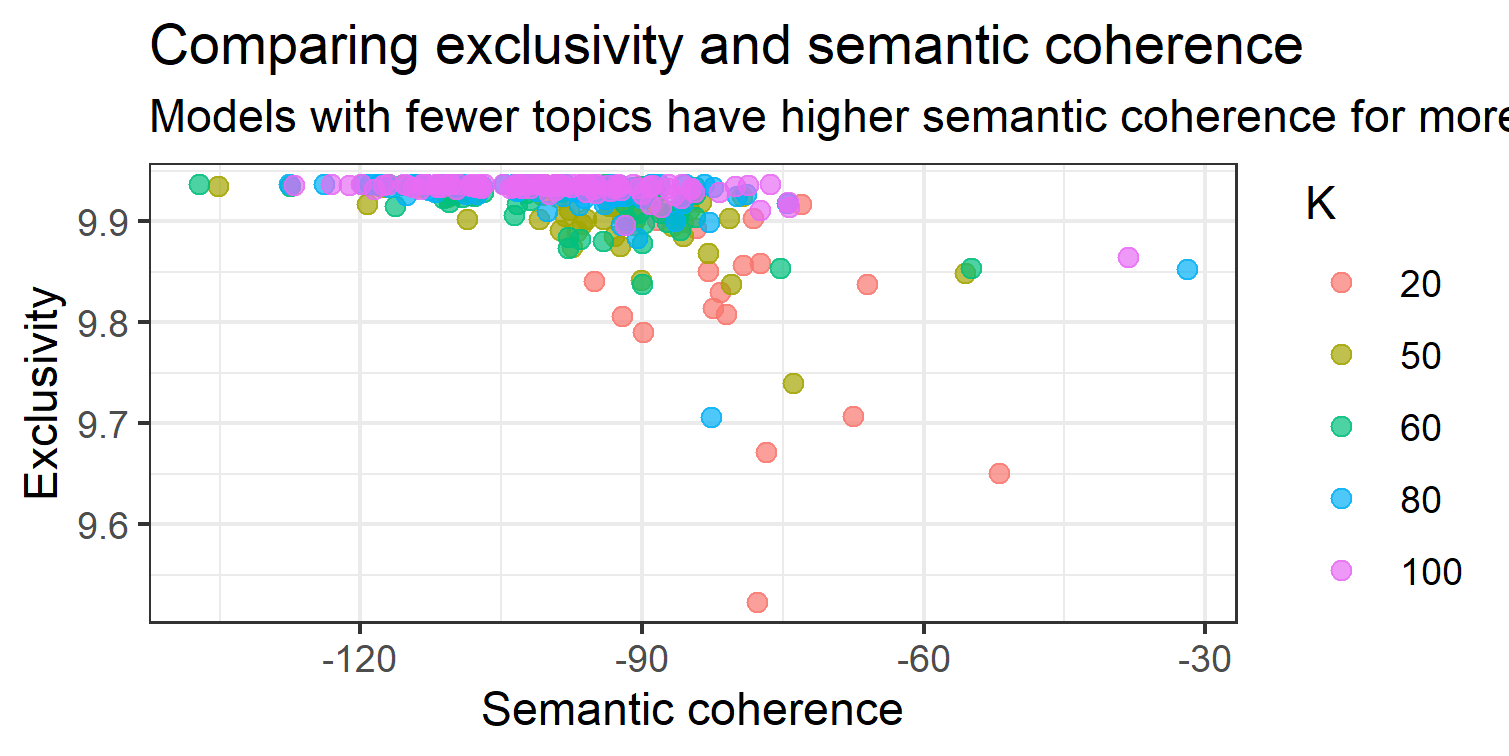
\includegraphics[width=.8\linewidth]{figs/exclusivity-vs-semantics.png}
	\caption{STM Results}
	\label{}
\end{figure}

However, ideally, we will also estimate a model high in both exclusivity and semantic coherence. Semantic coherence is high when the most probable words in a topic co-occur. Substantively, it maps on to topic quality and clarity. For example, we would expect ``Marx” and ``socialism” to co-occur in a well-fit model. Exclusivity captures the uniqueness of words to their topics. For example, it would be suboptimal if the word ``Marx” was a major contributing word to more than one topic because the more separate topics are from each other, the more we can learn from their presence/absence. There is a trade-off between semantic coherence and exclusivity.

\begin{figure} \centering
	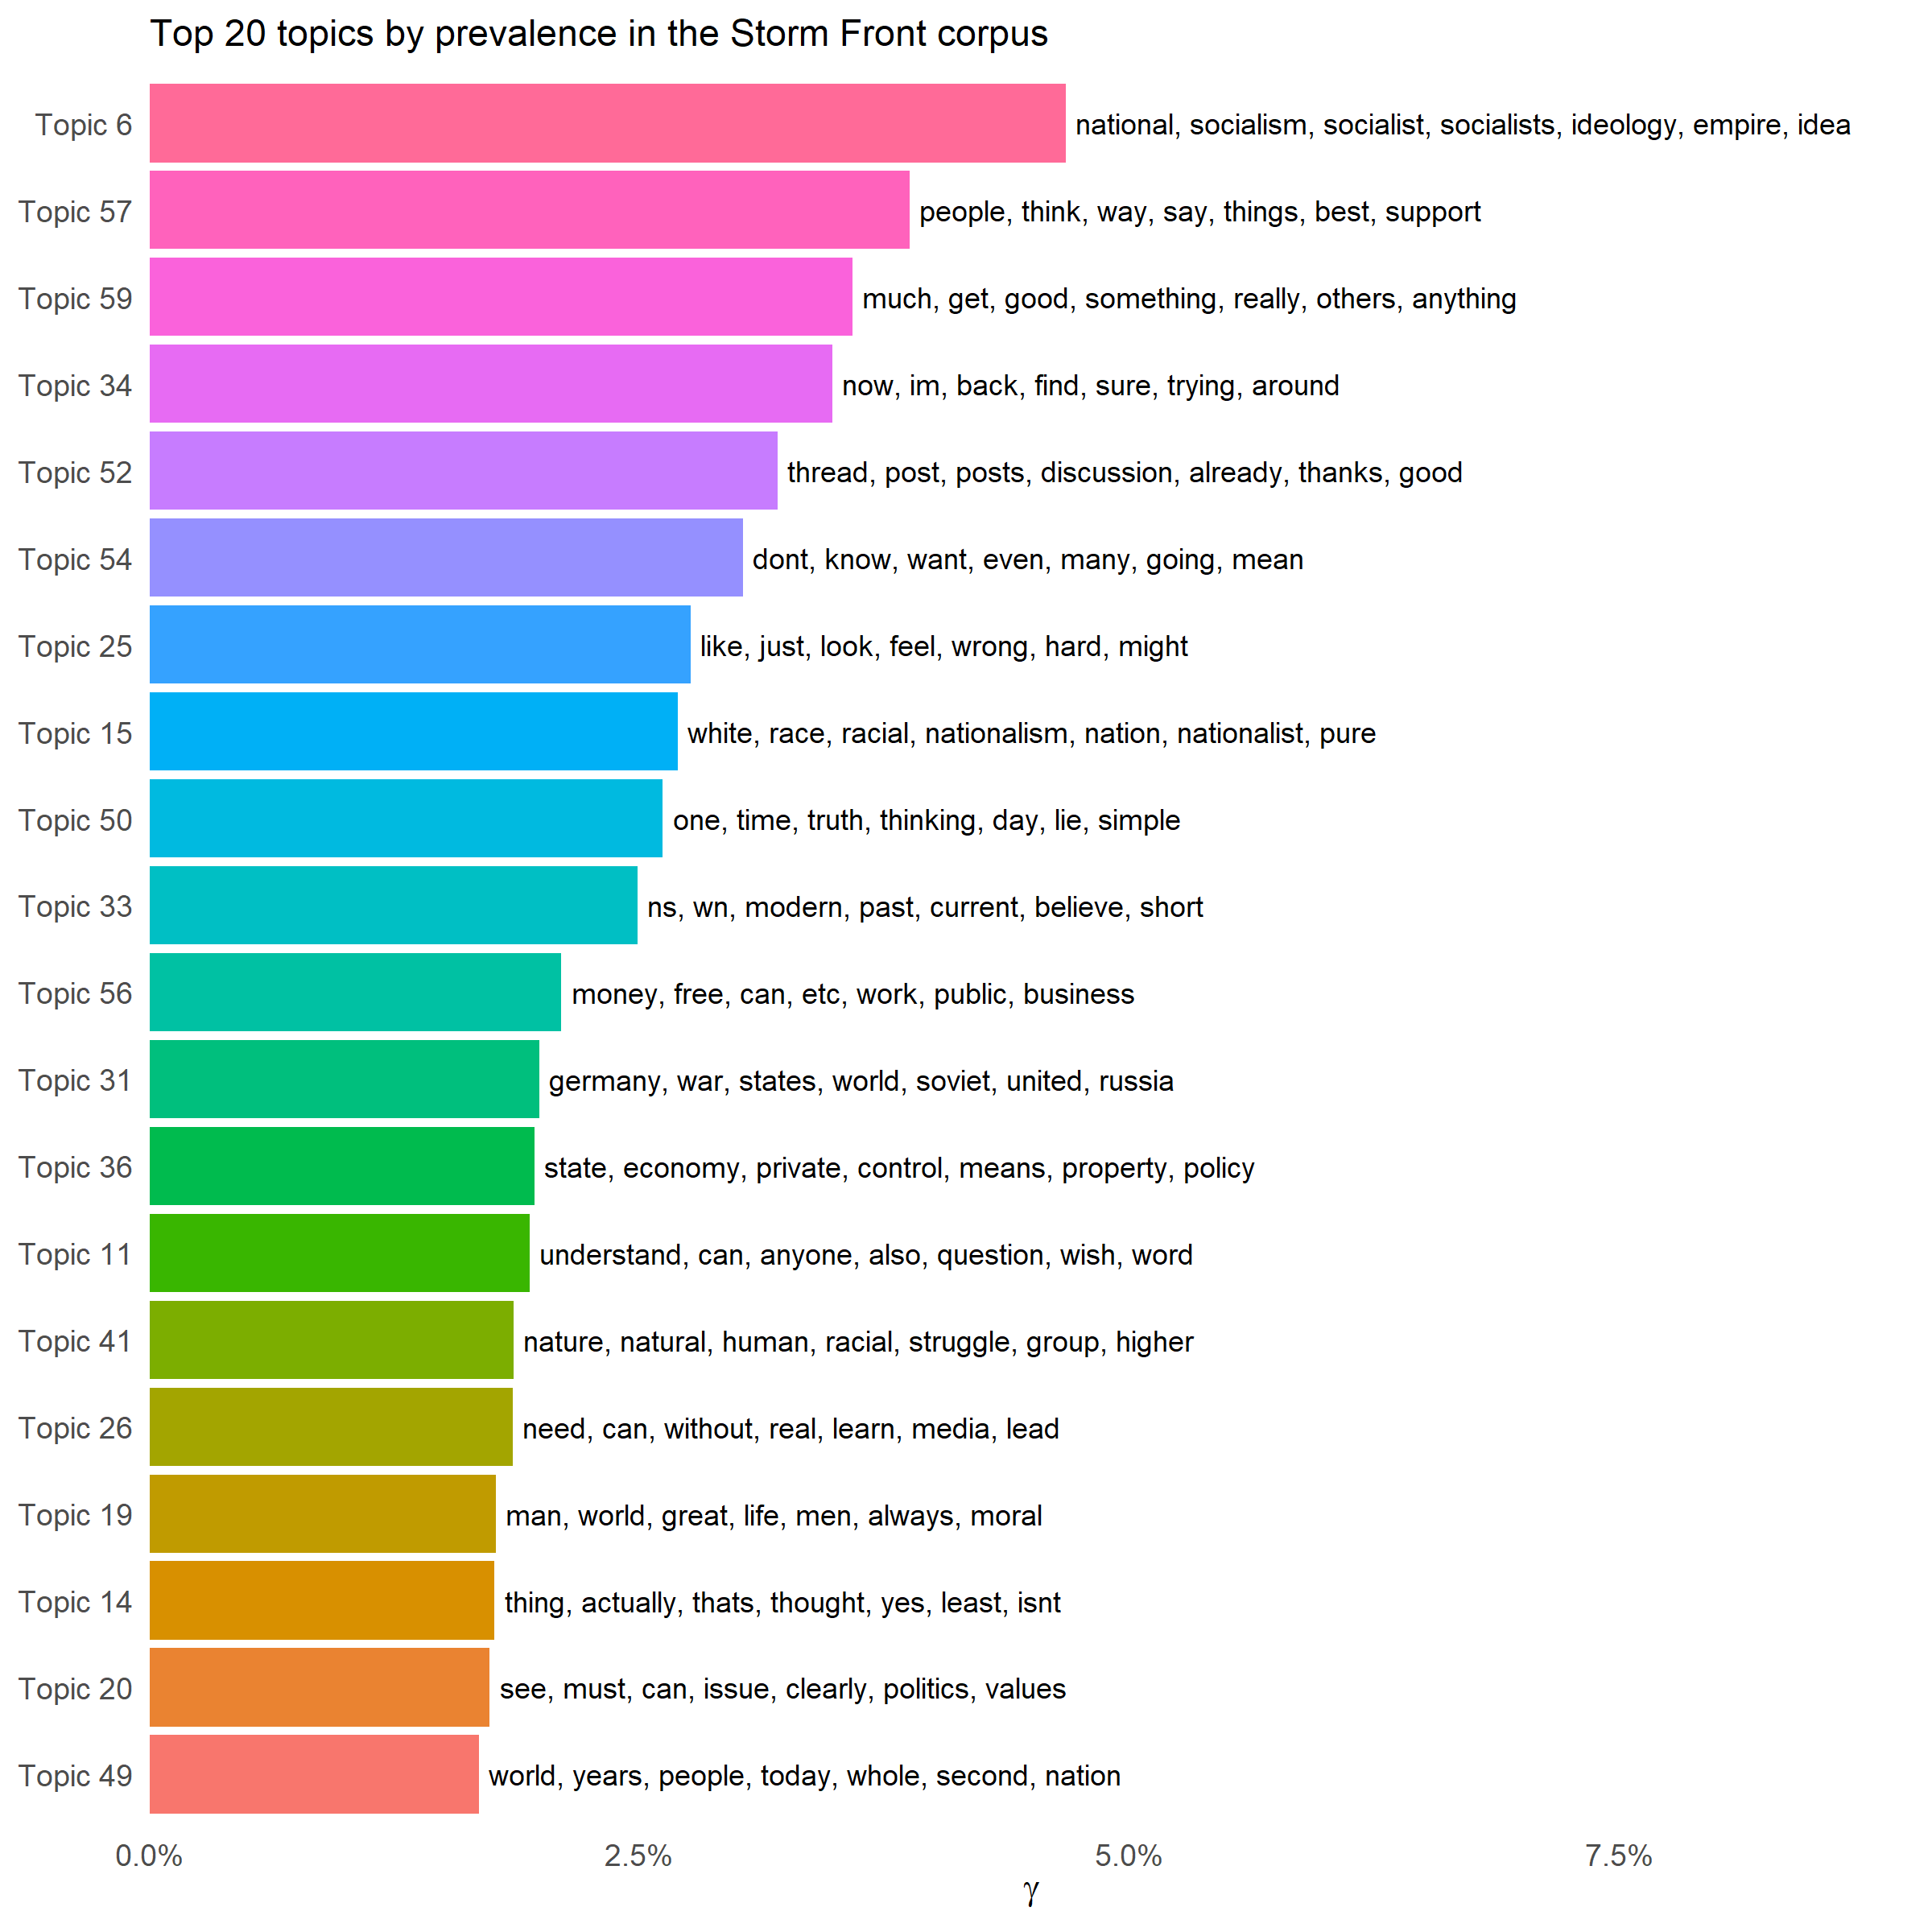
\includegraphics[width=.8\linewidth]{figs/top-20.png}
	\caption{STM Results}
	\label{}
\end{figure}

Given the clustering of estimates high in exclusivity and moderate in semantic coherence, I estimated a 60 topic model. The top 20 topics and the most prevalent words within those topics are shown in Figure 1 below, but a table with all 60 topics and prevalent words can be found in Appendix A.

As expected, given both the nature of StormFront.org and the Ideology and Philosophy subform, the most prevalent topic, Topic 6, is comprised of word-stems about nationalism, socialism, and ideology. Somewhat surprisingly, the next most-prevalent topic seems to focus on community; words like ``support" drive this topic. Language about race and white nationalism (wn) don't appear until the eighth most-prevalent topic. Readers will note that the words ``hate," ``dislike," words referencing violent actions (``kill," ``blow," ``pop," ``hit," ``hurt," etc.), and slurs are absent not only from the prevalent words in the top 20 topics, but from all 60 topics (Appendix A.)

To get a stronger idea of the sentiments contained within the corpus, I used the NRC Word-Emotion Association Lexicon (EmoLex) to uncover sentiment within the corpus (Mohammad and Turney 2010, 2013). The NRC EmoLex crowd-sourced the affective and emotional connotations of a variety of commonly-used words from native speakers. The results are striking and consistent with my prediction that the language used on StormFront.org will be quite positive. Indeed, the most frequently occurring sentiment is positivity.

\begin{figure} \centering
	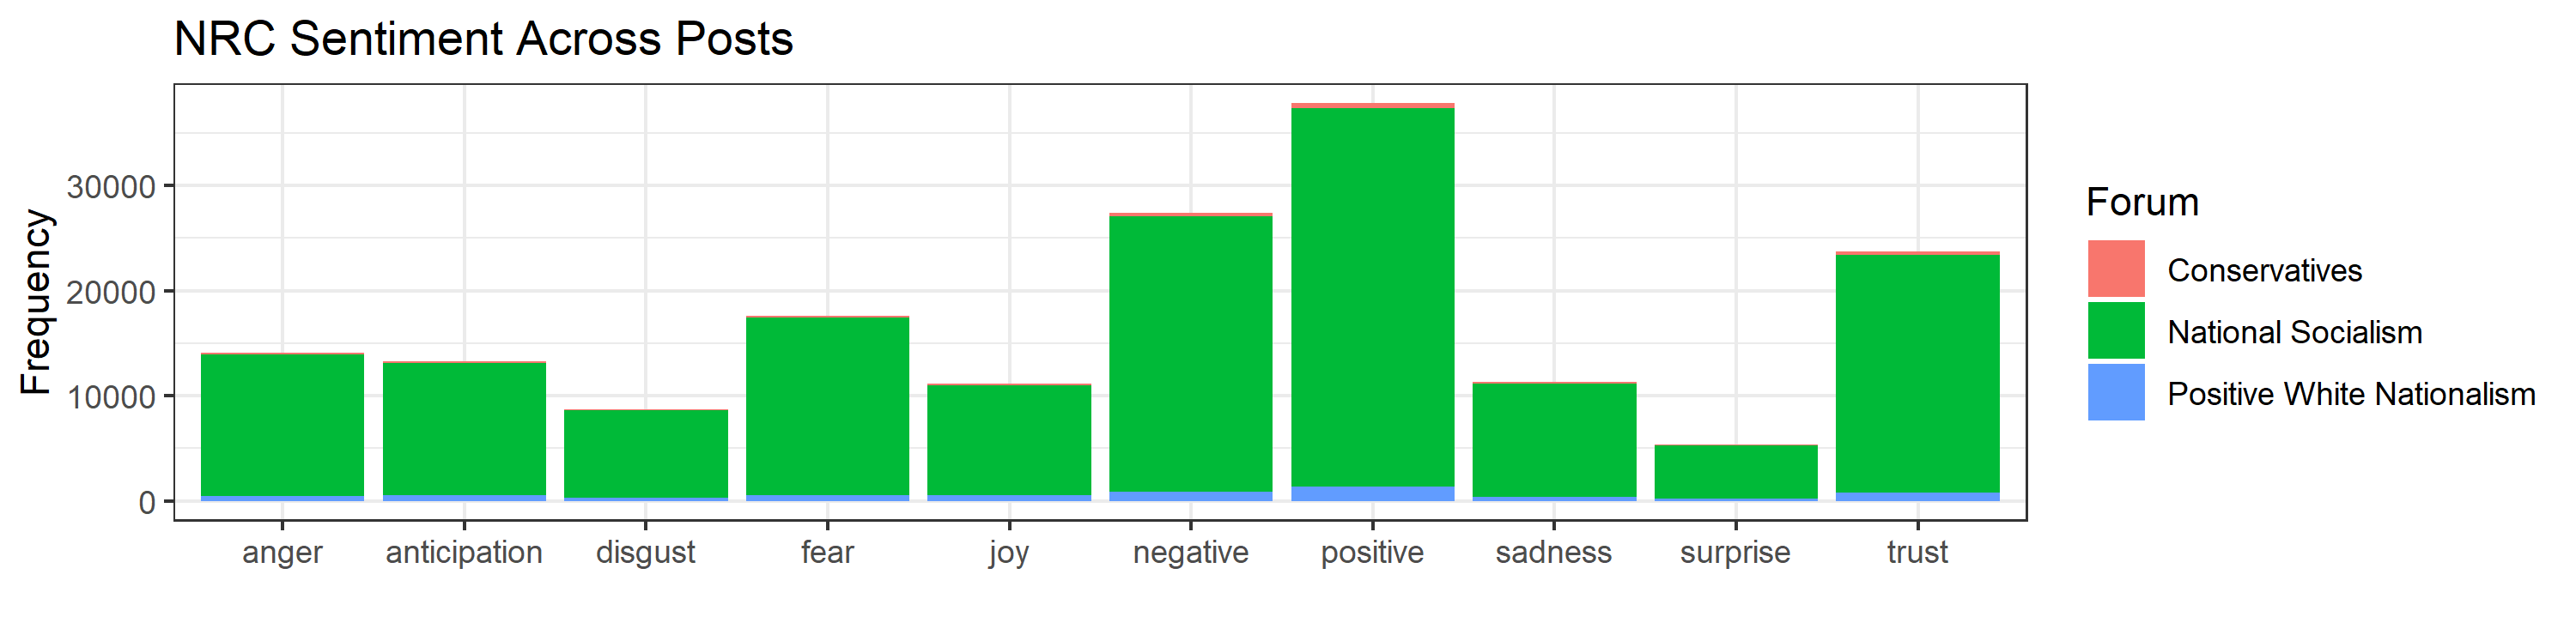
\includegraphics[width=.8\linewidth]{figs/sentiment_freq_all_words.png}
	\caption{NRC Sentiment Analysis}
	\label{}
\end{figure}


\section{Data In Context: StormFront.org the Virtual Space}
The banning of racial epithets on a white nationalist forum, created by the former Grand Wizard of the KKK for white nationalists, may seem counterintuitive to many readers. Indeed, StormFront.org is perhaps what comes to mind when they consider the darkest corners of the internet, yet topic and sentiment analysis reveal surprisingly tame language, given the topics being discussed. How do we square this with the acts of mass violence and digital harassment documented by qualitative scholars (Nagle 2016)? %%needed a scholarly version of "what gives?"

Bearing in mind that StormFront.org can be viewed by anyone and even has forums open to visitors where they can ask questions and share opposing viewpoints, this polished rhetoric seems less out of place than if the forum was closed to the public. StormFront.org appears to be not only a virtual community for white nationalists, but a recruitment tool for disaffected whites (De Koster and Houtman 2008; Bowman-Grieve 2009). As such, forum moderators are incentivized to ensure the forum appeals to those not already in the community. 

This raises important questions for the data-generating process of these scraped posts. What do they tell us about white nationalism as an ideology and white nationalists as individuals if they are intentionally curated to appeal to members of the outside world? In attempting to answer these questions, I wondered if there were avenues for discussion on the forum that could not be seen by the public. Perhaps forum moderators were able to so strongly enforce norms of polite, respectful language while keeping engagement up because the forum itself provided outlets for extreme and hateful language. To get a better understanding of this important context, I created an account on StormFront.org using a pseudonym and fake email address to preserve my safety.

In so doing, I discovered that a great deal of the activity on StormFront.org is hidden behind a membership wall. That is, it is unavailable to visitors without an account. If one joins the forum, one quickly sees that a great deal of activity occurs in ``Groups," which are private and separate from public-facing discussion boards. Many groups are run by site moderators and prominent users; access is invitation-only or, if you believe you should have access, you can submit references for gatekeepers to contact to verify your value to ``the cause." Members who are ``one post wonders" are rarely allowed into any groups, regardless of whether they are invitation-only or open to most users. Users are encouraged to post and participate in forum culture, to keep threads and groups active, and to exchange contact information to create real-life communities. While past work has noted that StormFront.org functions as a virtual community for disaffected whites (Bowman-Grieve 2009; Meddaugh and Kay 2009; Hartzell 2020), the mechanisms by which community is stimulated have remained hidden. The private network of social groups, private messaging, and the funnel from StormFront.org to private forums and chatrooms by invitation only are hidden from mere visitors.

All users who join the forum are sent an automated greeting message from Don Black. A few days later, notable white nationalist and ``Farm Belt Fuhrer" Gerhard Lauck sends along links to websites where new members can purchase translated Nazi materials popularized during the Third Reich. These include children's books like \textit{The Poisonous Mushroom} by Julius Streicher, war criminal and the publisher of \textit{Der Stürmer}.

It is clear that there is a communal understanding that some topics and sentiments are expressed only behind the wall of membership, in the safety of private social groups. Indeed, only a cursory search of the private social groups yields access to much more extreme content than is found on the publicly accessible forum. For example, there is a private social group called ``The Brotherhood" for ``those willing to do whatever it takes to secure the existence of our people. A group we may require in the future..." There is a private group for males only, with numerous threads dedicated to foreskin restoration because white nationalists consider circumcision genital mutilation. There is also a private group for ``Stormfronters Younger than 18," where the most popular threads include minors posting their ages, their ancestry, and debating ``the homosexual question."

This reality, heretofore not discussed by scholars of online white nationalism, has profound implications for our understanding not only of the data presented here, but of past work leveraging StormFront.org posts. Moderators have made both forum engagement and moderate language incentive compatible for users, because they have a private outlet for their more extreme sentiments. Users are at least somewhat cognizant that anything they say or write may be seen by the public or ``lurkers," who read the forums without joining. We should, therefore, not expect completely \textit{candid} speech from the public-facing forums; instead, we should expect a polished version of what white nationalists \textit{want} the world to know about them, underscored by strict posting guidelines. Still, using these data to obtain speech absent the confines of social desirability bias is still appropriate. Speech may not be entirely \textit{candid}, due to strict posting guidelines, but we have no reason to suspect that an inability to use slurs will change the underlying sentiment expressed by posters.

Further, the pseudonymous nature of the forum protects individual identities and allows for the sharing of genuine sentiment with limited ``real world" consequences. A similar approach was taken by Wu (2020) using the Economic Job Market Rumors Forum. The relatively niche nature of the forum, combined with the use of pseudonyms, lends credibility to the argument that users are more free to express their unaltered opinions in these contexts than on surveys and other information environments. Further, the forum is dedicated to white nationalist ideation. One could characterize the very purpose of StormFront.org as the pseudo-anonymous sharing of socially undesirable opinions. The public-facing forum has sub-forums dedicated to different topics such as revisionist history, culture, COVID-19, philosophy, politics, and white nationalist ideology, making it easier for users and researchers to obtain speech on specific topics.

Still, with the added context of private, member-only groups and loyalty hierarchies among members, we should not take the relative lack of vitriol in the data presented here as indicative of a lack of vitriol, racial-hatred, or extremism among white nationalist. Those sentiments appear to be relegated to private groups on the forum or funneled to private, invitation-only chatrooms, and private servers. We should instead view the data presented here - and, indeed, any data from StormFront's public forums - as indicative of the public image and rhetorical strategies used by white nationalists.

\section{Conclusion}
StormFront.org purports itself to be a rational, welcoming online community where discussing and enjoying whiteness is not taboo. Fitting a Structural Topic Model with a novel corpus of StormFront.org posts reveals this to be the dominant rhetoric on the forum; while racism is of course present on a forum devoted to white nationalist ideation, the language used is remarkably sterilized. Language about race and white nationalism (wn) don't appear until the eighth most-prevalent topic and the words ``hate," ``dislike," words referencing violent actions (``kill," ``blow," ``pop," ``hit," etc.), and slurs are altogether absent from the prevalent words in all 60 topics. Strict posting guidelines and community enforcement of discursive rules have scrubbed the forum of most recognizable forms of hate speech.

Existing work has either failed to contextualize this paucity of hate speech or attributed it to rhetorical strategy (Hartzell 2020); this article has gone a step farther, placing the public-facing forum in the broader context of StormFront.org as a virtual space, with private, member-only groups and chatrooms. Hateful language, calls to action, and the sharing of personal information are not only more common in these spaces, but encouraged.

The implications for future work are twofold. Firstly, topic modeling is a viable and useful method of analysis for forum data, with unique advantages over supervised-learning models. Future work may use the topics uncovered in this analysis as predictors of post length, violent language, expressions of interracial grievances, or other outcomes relevant to our understanding of political violence. Secondly, understanding the full context of a virtual space is critical to understanding the public-facing aspects of that virtual space. Beyond the case of StormFront, it is important that scholars of virtual communities and virtual extremism have a firm understanding of the digital ``field" in which they are conducting fieldwork, in order to appropriately frame and contextualize findings.


\section*{Works Cited}
\singlespace 
\begin{hangparas}{.25in}{1}

Berlet, C. and Mason, C., 2019. ``Swastikas in cyberspace 1: Ultra-Right White supremacy and antisemitism online.” \textit{In Trumping Democracy} (pp. 49-53). Routledge.
\\

Bowman-Grieve, Lorraine. 2009. ``Exploring ``Stormfront”: A virtual community of the radical right." \textit{Studies in conflict \& terrorism} 32, no. 11: 989-1007.
\\


Bright, Jonathan, Nahema Marchal, Bharath Ganesh, and Stevan Rudinac. 2022. ``How Do Individuals in a Radical Echo Chamber React to Opposing Views? Evidence from a Content Analysis of Stormfront." \textit{Human Communication Research} 48, no. 1: 116-145.
\\


Daniels, J., 2018. ``The algorithmic rise of the ``alt-right”." \textit{Contexts}, 17(1), pp.60-65.
\\


De Gibert, Ona, Naiara Perez, Aitor García-Pablos, and Montse Cuadros. 2018. ``Hate speech dataset from a white supremacy forum." arXiv preprint arXiv:1809.04444.
\\


De Koster, W. and Houtman, D. 2008. ``Stormfront is Like a Second Home To Me: On virtual community formation by right-wing extremists." \textit{Information, Communication \& Society,} 11(8), pp.1155-1176.
\\


Hartzell, S.L., 2020. ``Whiteness feels good here: interrogating white nationalist rhetoric on Stormfront.” \textit{Communication and Critical/Cultural Studies,} 17(2), pp.129-148.
\\


Kim, T. K. 2005. ``Electronic storm: Stormfront grows a thriving neo-nazi community." Intelligence Report., Southern Poverty Law Center.
\\


Moberg, S.P., Krysan, M. and Christianson, D. 2019. ``Racial attitudes in America." \textit{Public Opinion Quarterly}, 83(2), pp.450-471.
\\


Nagle, Angela. 2016. \textit{Kill all normies: Online culture wars from 4chan and Tumblr to Trump and the alt-right.} John Hunt Publishing.
\\


Nederhof, A.J., 1985. ``Methods of coping with social desirability bias: A review.” \textit{European journal of social psychology}, 15(3), pp.263-280.
\\


Meddaugh, Priscilla Marie, and Jack Kay. 2009. ``Hate speech or ``reasonable racism?” The other in Stormfront." Journal of Mass Media Ethics 24, no. 4: 251-268.
\\


Roberts, Margaret E., Brandon M. Stewart, Dustin Tingley, and Edoardo M. Airoldi. 2013. ``The structural topic model and applied social science." In \textit{Advances in neural information processing systems workshop on topic models: computation, application, and evaluation}, vol. 4, pp. 1-20.
\\


Thompson, K.C., 2001. ``Watching the Stormfront: White nationalists and the building of community in cyberspace.” \textit{Social Analysis: The International Journal of Social and Cultural Practice,} 45(1), pp.32-52.
\\


\textit{Welcome: Guidelines for Posting}. Stormfront.org. Retreived on 4/25/2022. https://www.stormfront.org/forum/t4359/
\\


Wojcieszak, M., 2010. ```Don’t talk to me’: Effects of ideologically homogeneous online groups and politically dissimilar offline ties on extremism.” \textit{New Media \& Society,} 12(4), pp.637-655.
\\


Wu, A.H., 2020. ``Gender Bias among Professionals: An Identity-Based Interpretation." \textit{Review of Economics and Statistics}, 102(5), pp.867-880.
\end{hangparas}


\section*{Appendix A}
%%That table HERE
\begin{table}[H]
	\begin{adjustbox}{width=1\textwidth}
		\begin{tabular}{lll}
			\multicolumn{1}{c}{\textbf{Topic}} & \multicolumn{1}{c}{\textbf{Expected Topic Proportion}} & \multicolumn{1}{c}{\textbf{Top 7 Terms}}                            \\
			Topic 6                            & 0.047                                                  & national, socialism, socialist, socialists, ideology, empire, idea  \\
			Topic 57                           & 0.039                                                  & people, think, way, say, things, best, support                      \\
			Topic 59                           & 0.036                                                  & much, get, good, something, really, others, anything                \\
			Topic 34                           & 0.035                                                  & now, im, back, find, sure, trying, around                           \\
			Topic 52                           & 0.032                                                  & thread, post, posts, discussion, already, thanks, good              \\
			Topic 54                           & 0.030                                                  & dont, know, want, even, many, going, mean                           \\
			Topic 25                           & 0.028                                                  & like, just, look, feel, wrong, hard, might                          \\
			Topic 15                           & 0.027                                                  & white, race, racial, nationalism, nation, nationalist, pure         \\
			Topic 50                           & 0.026                                                  & one, time, truth, thinking, day, lie, simple                        \\
			Topic 33                           & 0.025                                                  & ns, wn, modern, past, current, believe, short                       \\
			Topic 56                           & 0.021                                                  & money, free, can, etc, work, public, business                       \\
			Topic 31                           & 0.020                                                  & germany, war, states, world, soviet, united, russia                 \\
			Topic 36                           & 0.020                                                  & state, economy, private, control, means, property, policy           \\
			Topic 11                           & 0.019                                                  & understand, can, anyone, also, question, wish, word                 \\
			Topic 41                           & 0.019                                                  & nature, natural, human, racial, struggle, group, higher             \\
			Topic 26                           & 0.019                                                  & need, can, without, real, learn, media, lead                        \\
			Topic 19                           & 0.018                                                  & man, world, great, life, men, always, moral                         \\
			Topic 14                           & 0.018                                                  & thing, actually, thats, thought, yes, least, isnt                   \\
			Topic 20                           & 0.017                                                  & see, must, can, issue, clearly, politics, values                    \\
			Topic 49                           & 0.017                                                  & world, years, people, today, whole, second, nation                  \\
			Topic 2                            & 0.017                                                  & hitler, adolf, hitlers, speech, fact, later, made                   \\
			Topic 27                           & 0.016                                                  & us, let, believe, future, truly, enemies, come                      \\
			Topic 7                            & 0.016                                                  & point, however, seems, consider, different, believe, seem           \\
			Topic 58                           & 0.016                                                  & capitalism, communism, marxist, marx, marxism, fascism, class       \\
			Topic 45                           & 0.016                                                  & chapter, fight, existence, volume, hands, must, purity              \\
			Topic 37                           & 0.016                                                  & never, use, used, ive, seen, side, propaganda                       \\
			Topic 38                           & 0.015                                                  & party, political, nsdap, taken, program, organization, social       \\
			Topic 48                           & 0.015                                                  & new, old, revolution, republic, revolutionary, time, red            \\
			Topic 53                           & 0.015                                                  & aryan, european, culture, peoples, europe, blood, germanic          \\
			Topic 40                           & 0.015                                                  & well, said, die, put, done, re, saying                              \\
			Topic 22                           & 0.015                                                  & movement, ideas, term, call, cause, idea, views                     \\
			Topic 17                           & 0.014                                                  & american, america, history, black, americans, early, upon           \\
			Topic 46                           & 0.014                                                  & make, sense, makes, still, common, problems, fact                   \\
			Topic 47                           & 0.014                                                  & law, rights, right, must, state, demand, duty                       \\
			Topic 10                           & 0.014                                                  & nazi, nazis, nazism, communists, wasnt, nationalism, socialists     \\
			Topic 44                           & 0.014                                                  & power, form, freedom, democracy, political, leadership, rule        \\
			Topic 3                            & 0.013                                                  & first, better, two, comes, understanding, action, aware             \\
			Topic 23                           & 0.013                                                  & either, certain, terms, ie, much, rest, class                       \\
			Topic 12                           & 0.013                                                  & government, country, people, line, good, citizens, much             \\
			Topic 39                           & 0.013                                                  & course, perhaps, case, indeed, example, far, completely             \\
			Topic 4                            & 0.012                                                  & children, working, care, million, family, years, women              \\
			Topic 9                            & 0.012                                                  & whites, races, fight, taking, means, victory, nonwhites             \\
			Topic 21                           & 0.012                                                  & religion, christianity, christian, god, religious, speak, faith     \\
			Topic 13                           & 0.012                                                  & read, mein, book, reading, also, link, wrote                        \\
			Topic 42                           & 0.012                                                  & system, economic, capitalist, took, based, systems, view            \\
			Topic 51                           & 0.011                                                  & jews, jewish, jew, jesus, liberal, fact, lies                       \\
			Topic 55                           & 0.011                                                  & german, people, workers, germans, germany, international, destroyed \\
			Topic 5                            & 0.011                                                  & community, shall, within, purpose, society, individual, order       \\
			Topic 32                           & 0.011                                                  & another, points, tell, made, forum, ill, correct                    \\
			Topic 24                           & 0.010                                                  & kampf, original, interested, written, quotes, thoughts, mention     \\
			Topic 30                           & 0.010                                                  & true, right, left, stated, false, towards,                          \\
			Topic 8                            & 0.009                                                  & name, century, exactly, simply, came, matters, next                 \\
			Topic 28                           & 0.009                                                  & part, opinion, ideology, success, argument, death, greater          \\
			Topic 16                           & 0.009                                                  & every, person, quite, certainly, single, entire, fully              \\
			Topic 60                           & 0.009                                                  & place, long, become, fear, people, behind, even                     \\
			Topic 43                           & 0.009                                                  & last, reason, edited, pm, theres, real, made                        \\
			Topic 18                           & 0.008                                                  & go, found, enemy, spirit, words, civilization, western              \\
			Topic 29                           & 0.008                                                  & reich, third, history, german, youth, military, army                \\
			Topic 35                           & 0.006                                                  & agree, folk, der, im, folks, problem, nation                        \\
			Topic 1                            & 0.003                                                  & little, nietzsche, und, von, war, im, philosophy                   
		\end{tabular}
	\end{adjustbox}
	\caption{Sixty-Topic STM of StormFront.org Corpus} 
	\label{}
\end{table}


\end{document}